% Exercise Template
% A LaTeX template for typesetting exercise in Persian.
% Based on Sharif CE template

\documentclass[12pt]{exam}

\usepackage{setspace}
\usepackage{listings}
\usepackage{graphicx,subfigure,wrapfig}
\usepackage{multirow}
\usepackage{booktabs}
\usepackage{amssymb,amsmath}
\usepackage{xcolor}
\usepackage[hidelinks]{hyperref}
\usepackage[margin=20mm]{geometry}
\usepackage{xepersian}
\settextfont[
  Path = ./assets/fonts/,
  BoldFont = Vazirmatn-Bold.ttf
]{Vazirmatn-Regular.ttf}

\newcommand{\class}{درس برنامه‌سازی وب}
\newcommand{\term}{نیم‌سال اول ۰۵-۰۶}
\newcommand{\college}{دانشکده مهندسی کامپیوتر}
\newcommand{\prof}{استاد: جناب آقای پروفسور علی ابریشمی}
\newcommand{\student}{نیما حکمتی فرید ۴۰۲۱۰۵۹۲۱}

\singlespacing
\parindent 0ex

\lstset{
  basicstyle=\ttfamily\small,
  keywordstyle=\textbf,
  identifierstyle=,
  commentstyle=\color{gray},
  stringstyle=\ttfamily,
  numberstyle=\footnotesize,
  showstringspaces=false
}

\begin{document}

% These commands set up the running header on the top of the exam pages
\pagestyle{head}
\firstpageheader{}{}{}
\runningheader{صفحه \thepage\ از \numpages}{}{\class}
\runningheadrule
\begin{tabular*}{\textwidth}{@{\extracolsep{\fill}} r c}
\multicolumn{2}{c}{\textbf{به نام خدا}}\vspace{6pt}\\
\textbf{\class} & \multirow{5}{*}{
\includegraphics[width=2.4cm]{assets/images/logo.png}} \\
\textbf{\term} & \\
\textbf{\prof} & \\
\textbf{\student} & \\
\textbf{\college} & \\
\end{tabular*}\\

\rule[1ex]{\textwidth}{.1pt}
\textbf{گزارش پروژه تمرین اول: بازآفرینی سامانه کتابخوان دیجیتال طاقچه}

\rule[1ex]{\textwidth}{.1pt}
\vspace{0pt}

\begin{questions}

\question
\textbf{معرفی سازنده و اهداف پروژه:}
\\
این پروژه در چارچوب تمرین اول درس برنامه‌سازی وب دانشکده مهندسی کامپیوتر دانشگاه صنعتی شریف در \term\ زیر نظر \prof\ پیاده‌سازی شده است.
\\
\textbf{مشخصات توسعه‌دهنده:} نیما حکمتی فرید، شماره دانشجویی ۴۰۲۱۰۵۹۲۱.
\\
\textbf{اهداف محوری پروژه:}
\begin{itemize}
    \item بازآفرینی تجربه کاربری، ساختار چیدمان و تعاملات سامانه محبوب کتابخوان \textbf{طاقچه}.
    \item تسلط عمیق بر استانداردهای اصیل وب (\lr{Pure HTML5}، \lr{CSS3} نوین و \lr{Vanilla JavaScript}).
    \item پایبندی مطلق به اصل عدم وابستگی (\lr{Zero Dependencies})؛ پروژه بدون استفاده از هیچ‌گونه فریم‌ورک (\lr{React, Vue, Tailwind, Bootstrap}) یا کتابخانه جانبی توسعه یافته است.
    \item ارائه یک تجربه تک‌صفحه‌ای پیوسته (\lr{SPA}) با مسیریابی مبتنی بر \lr{Hash}، سیستم احراز هویت با حالت اختصاصی برای هر کاربر، ذخیره‌سازی محلی (\lr{LocalStorage}) و طراحی واکنش‌گرا برای عرض‌های ۳۶۰، ۷۶۸ و ۱۴۴۰ پیکسل.
\end{itemize}

\question
\textbf{تصاویر مرجع طاقچه با تاریخ مشاهده (بند ۱ و ۵ راهنما):}
\\
جهت انطباق دقیق هویت بصری، سلسله‌مراتب داده‌ها و جریان کاربری، سه نمای محوری از سامانه اصلی طاقچه در تاریخ \textbf{۱۴ آبان ۱۴۰۵} مستندسازی و بررسی گردید:
\begin{enumerate}
    \item \textbf{صفحه اصلی (\lr{Home}):} شامل ساختار سربرگ با فیلد جستجوی زنده، ناوبری دسته‌بندی‌ها، اسلایدر بنرهای مناسبتی، قفسه‌های افقی کتاب‌ها، بخش پرفروش‌ترین‌ها و فوتر غنی با اطلاعات کامل.
    \item \textbf{فهرست و کاوش کتاب‌ها (\lr{Catalog}):} شامل فیلترهای چندمعیاره در سایدبار (دسته‌بندی، نوع محتوا اعم از متنی و صوتی، فیلتر رایگان، بازه قیمت)، مرتب‌سازی براساس محبوب‌ترین، جدیدترین و قیمت، و گرید کارت‌های کتاب.
    \item \textbf{صفحه جزییات و مشخصات کتاب (\lr{Book Details}):} شامل کارت جلد و مشخصات فنی (شابک، ناشر، سال نشر، تعداد صفحات)، دکمه‌های دریافت کتاب و نمونه‌خوانی، معرفی متنی، و قفسه کتاب‌های مرتبط.
\end{enumerate}

\begin{figure}[htbp]
\centering
\subfigure[صفحه اصلی طاقچه (مشاهده: ۱۴ آبان ۱۴۰۵)]{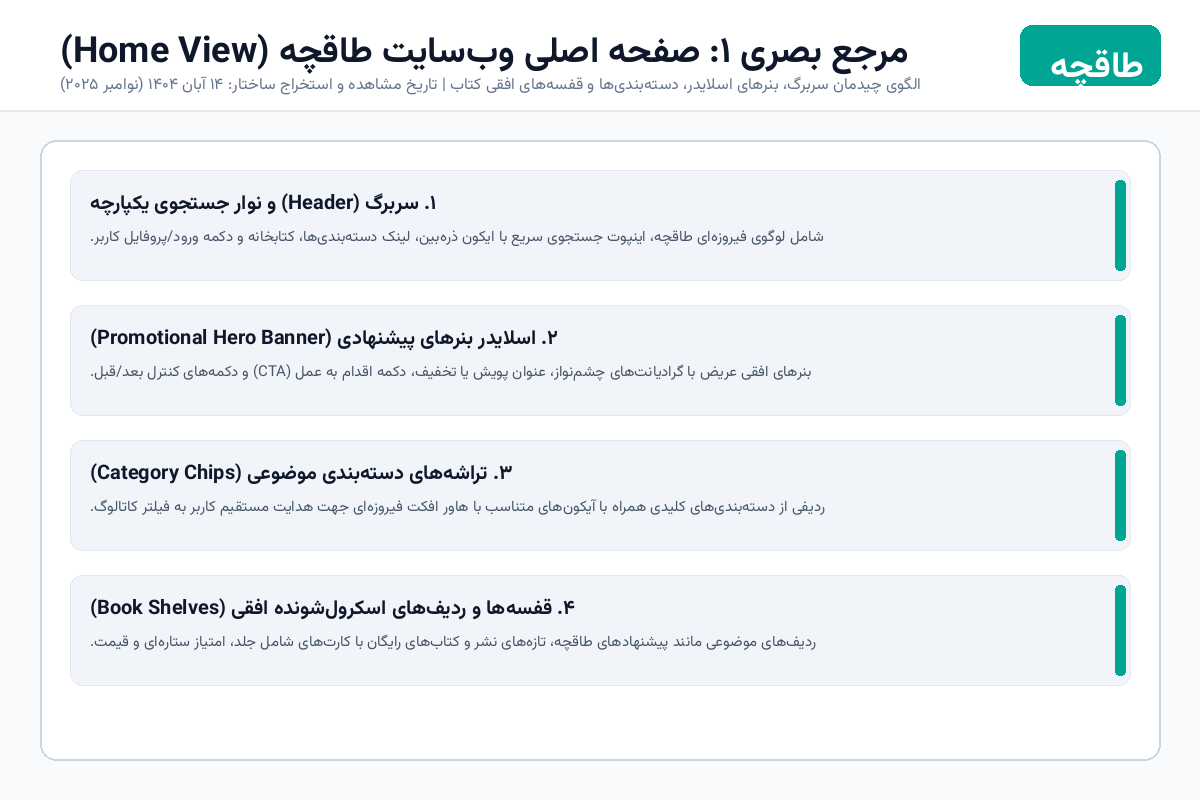
\includegraphics[width=0.31\textwidth]{assets/references/reference-taaghche-home.png}}
\hfill
\subfigure[فهرست و جستجوی طاقچه (مشاهده: ۱۴ آبان ۱۴۰۵)]{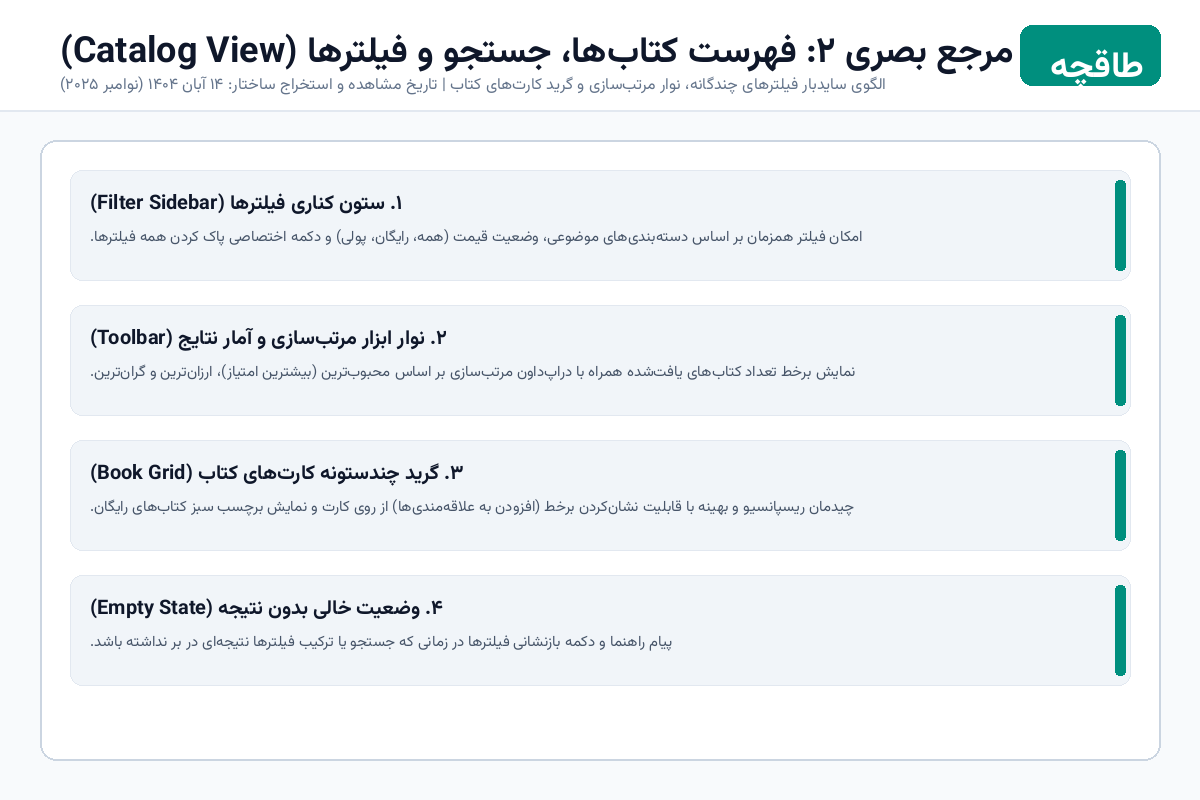
\includegraphics[width=0.31\textwidth]{assets/references/reference-taaghche-catalog.png}}
\hfill
\subfigure[صفحه جزییات کتاب در طاقچه (مشاهده: ۱۴ آبان ۱۴۰۵)]{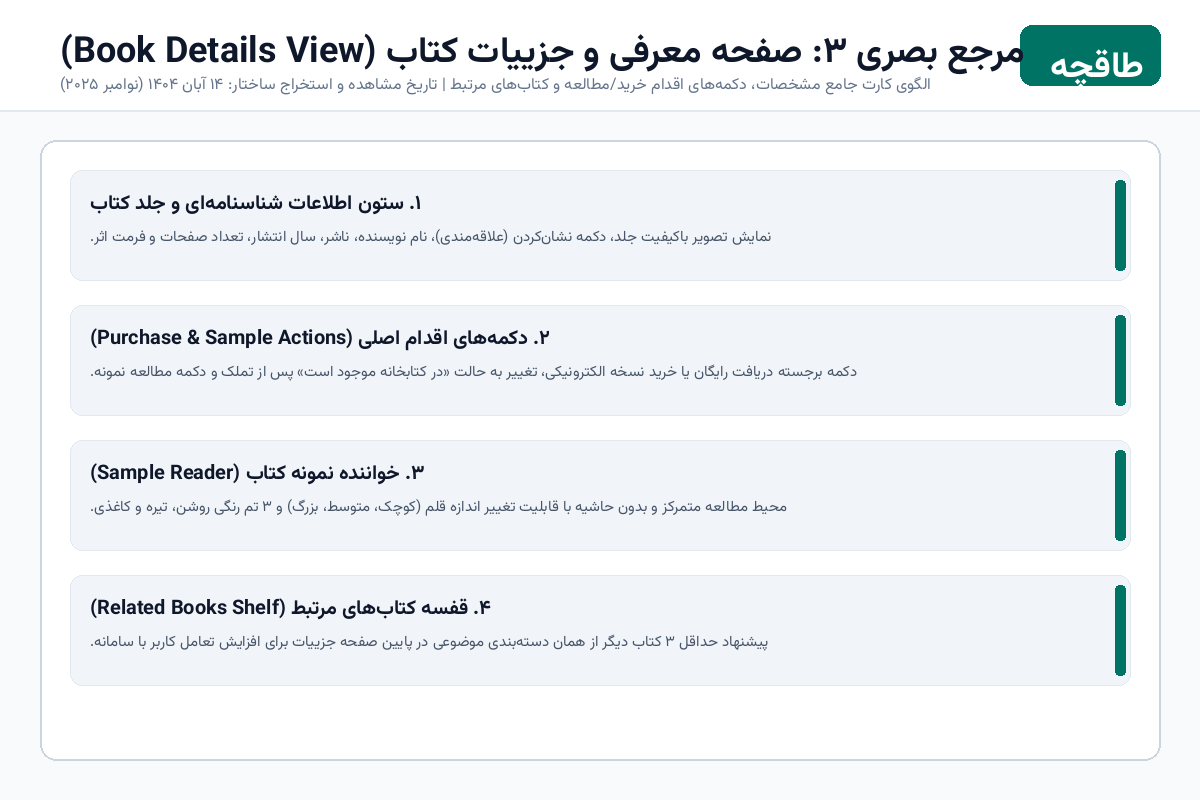
\includegraphics[width=0.31\textwidth]{assets/references/reference-taaghche-details.png}}
\caption{تصاویر مرجع از وب‌سایت اصلی طاقچه (استخراج‌شده در ۱۴ آبان ۱۴۰۵)}
\end{figure}

\question
\textbf{روند واقعی ساخت، معماری و تصمیمات پیاده‌سازی:}
\begin{itemize}
    \item \textbf{ساختار ماژولار و فایل‌ها:}
    پروژه در پوشه‌بندی استاندارد توسعه یافته است:
    \begin{itemize}
        \item \texttt{index.html}: نشانی‌گذاری معنایی (\lr{Semantic HTML5})، با استفاده از تگ‌های \texttt{header}، \texttt{nav}، \texttt{main}، \texttt{section}، \texttt{aside} و \texttt{footer}.
        \item \texttt{css/style.css}: طراحی مدرن با متغیرهای طراحی (\lr{CSS Custom Properties}) برای مدیریت دو تم روشن و تاریک، سیستم چیدمان \lr{CSS Grid} و \lr{Flexbox}، انیمیشن‌های روان و استانداردهای رسانه‌ای (\lr{Media Queries}).
        \item \texttt{js/books.js}: پایگاه داده داده‌محور کتاب‌ها (۲۴ کتاب در دسته‌های رمان، روانشناسی، مدیریت، تاریخ، فلسفه، علمی و شعر همراه با متن نمونه چندبخشی برای خواننده).
        \item \texttt{js/app.js}: منطق کامل برنامه، درایور ناوبری \lr{Hash Routing}، کنترلر احراز هویت، مدیریت قفسه‌ها، موتور جستجو و فیلتر، و رابط کتابخوان.
    \end{itemize}

    \item \textbf{مسیریابی تک‌صفحه‌ای (\lr{Hash-based SPA Router}):}
    با پایش رخداد \texttt{hashchange}، بدون بارگذاری مجدد صفحه، نماهای \texttt{\#home}، \texttt{\#catalog}، \texttt{\#book/:id}، \texttt{\#reader/:id}، \texttt{\#library}، \texttt{\#login}، \texttt{\#cart} و \texttt{\#profile} مدیریت و متناسب با شناسه پارامتریک رندر می‌شوند.

    \item \textbf{مدیریت تم دوگانه (\lr{Light / Dark Mode}):}
    سیستم رنگ‌ها بر اساس متغیرهای سی‌اس‌اس (\lr{Variables}) با تغییر کلاس \texttt{dark-theme} روی تگ ریشه \texttt{html} پیاده‌سازی شده و انتخاب کاربر در حافظه مرورگر پایدار می‌ماند.
\end{itemize}

\question
\textbf{ساختار داده‌ها، منطق جستجو، فیلترها و ذخیره‌سازی حالت:}
\begin{itemize}
    \item \textbf{ساختار داده کتاب‌ها:}
    هر شیء کتاب در آرایه داده‌ها شامل شناسه‌های یکتا، عنوان فارسی و انگلیسی، نویسنده، مترجم، ناشر، سال نشر، شابک (\lr{ISBN})، تعداد صفحه، رتبه‌بندی، قیمت ریالی، تخفیف، نوع محتوا (\lr{text} یا \lr{audio})، تگ‌ها، خلاصه‌ی معرفی و محتوای فصول چندگانه نمونه است.

    \item \textbf{موتور جستجوی چندفیلدی با نرمال‌سازی فارسی:}
    تابع جستجو کاراکترهای عربی و فارسی (ی و ک) و اعراب را نرمال کرده و به صورت همزمان فیلدهای عنوان، نویسنده، مترجم و ناشر را با عبارات چندکلمه‌ای تطبیق می‌دهد. سیستم جستجوی پیش‌بینی‌کننده با منوی بازشونده زنده در هنگام تایپ کلمات کلیدی، پیشنهادهای سریع به کاربر ارائه می‌دهد.

    \item \textbf{فیلترهای ترکیبی در کاتالوگ:}
    کاربر می‌تواند به صورت همزمان فیلتر دسته‌بندی موضوعی، نوع کتاب (الکترونیکی / صوتی)، کتاب‌های رایگان، بازه قیمتی دلخواه و ترتیب نمایش (پربازدیدترین، گران‌ترین، ارزان‌ترین و جدیدترین) را اعمال نماید.

    \item \textbf{تفکیک ایزوله حالت برای هر کاربر (\lr{Per-User State Storage}):}
    اطلاعات کاربری، کتابخانه، علاقه‌مندی‌ها و موقعیت نشانه‌گذاری کتابخوان برای هر کاربر بر اساس شماره تماس در کلید \texttt{taaghche\_users\_store} در \lr{LocalStorage} تفکیک شده است. با خروج کاربر (\lr{Logout})، وضعیت فعال سیستم ریست می‌شود و با ورود مجدد هر شماره، داده‌های پیشین همان کاربر به صورت مستقل بارگذاری می‌گردد.
\end{itemize}

\question
\textbf{چالش‌های فنی، راهکارها و جزئیات رفع اشکال:}
\begin{itemize}
    \item \textbf{واکنش‌گرایی سربرگ و خواننده در عرض ۳۶۰ پیکسل:}
    در عرض‌های کوچک موبایل، تجمع دکمه‌های جستجو، سبد خرید، حساب کاربری و سوییچ تم موجب فشردگی و شکست عناصر می‌شد.
    \\
    \textbf{راهکار:} پیاده‌سازی منوی کشویی جانبی (\lr{Mobile Drawer})، نوار دسترسی سریع پایین صفحه (\lr{Bottom Navigation Bar}) و بازطراحی سربرگ کتابخوان در دو ردیف انعطاف‌پذیر با \lr{Flexbox wrap} و کنترل لمسی پدینگ‌ها و دکمه‌ها.

    \item \textbf{ایزولاسیون کامل نشست‌های کاربری:}
    نگهداری داده‌ها در یک کلید مشترک موجب تداخل کتابخانه‌های کاربران مختلف می‌شد.
    \\
    \textbf{راهکار:} ایجاد لایه ذخیره‌سازی داده نقشه‌برداری‌شده (\lr{User-to-State Map}) که شماره موبایل را کلید جدول کاربران قرار داده و هنگام خروج، کانتکست فعال پاکسازی شده و حریم خصوصی محفوظ می‌ماند.

    \item \textbf{کتابخوان با شخصی‌سازی کامل:}
    امکان تغییر اندازه فونت، فاصله خطوط، عرض متن، انتخاب تم مطالعه (روشن، تیره، کاغذ قدیمی/سپیا) و ثبت نشانک با درج درصدی موقعیت اسکرول به صورت کامپوننت بومی با عملکرد روان پیاده‌سازی گردید.
\end{itemize}

\question
\textbf{ماتریس آزمون‌های کارکردی بخش ۶ صورت تمرین:}
\\
تمامی آزمون‌های تعریف‌شده در بخش ۶ صورت تمرین به صورت دقیق مورد ارزیابی قرار گرفتند و نتایج در جدول زیر مستند شده است:

\begin{table}[htbp]
\centering
\footnotesize
\begin{tabular}{p{0.08\textwidth} p{0.22\textwidth} p{0.27\textwidth} p{0.25\textwidth} c}
\toprule
\textbf{کد سناریو} & \textbf{عنوان آزمون} & \textbf{مراحل اجرایی} & \textbf{نتیجه مشاهده‌شده} & \textbf{وضعیت} \\
\midrule
TC-01 & واکنش‌گرایی در عرض‌های استاندارد & تغییر ویوپورت به ۳۶۰، ۷۶۸ و ۱۴۴۰ پیکسل & انطباق کامل بدون اسکرول افقی، دراور موبایل و هدر ۲ردیفه & موفق $\checkmark$ \\
\addlinespace
TC-02 & آزمون جستجو و فیلترها & جستجوی «کلیدر» و اعمال فیلتر رمان و رایگان & پالایش فوری داده‌ها بدون تاخیر و تطبیق همزمان چند شرط & موفق $\checkmark$ \\
\addlinespace
TC-03 & آزمون خرید و کتابخانه & ورود، افزودن کتاب به سبد و تسویه‌حساب & انتقال آنی کتاب به کتابخانه من با برچسب خریداری‌شده & موفق $\checkmark$ \\
\addlinespace
TC-04 & خواننده کتاب و نشانه‌گذاری & باز کردن نمونه کتاب، تنظیم قلم و رنگ پس‌زمینه & ذخیره دقیق موقعیت مطالعه در حافظه و بازیابی در مراجعه بعد & موفق $\checkmark$ \\
\addlinespace
TC-05 & چندکاربری و پایداری وضعیت & ورود با شماره A و ذخیره نشانک، خروج، ورود با شماره B & پاک‌شدن وضعیت با خروج، استقلال کامل داده‌های هر کاربر & موفق $\checkmark$ \\
\bottomrule
\end{tabular}
\caption{ماتریس ارزیابی و نتایج آزمون‌های جامع پروژه}
\end{table}

\question
\textbf{وضعیت نهایی قابلیت‌ها، تصاویر پیاده‌سازی و مراجع:}
\begin{itemize}
    \item \textbf{پوشش ۱۰۰ درصدی نیازمندی‌ها:} تمامی موارد خواسته‌شده در فاز اول پروژه شامل سربرگ تعاملی، قفسه‌های متنوع، کاتالوگ با فیلترها و مرتب‌سازی، صفحه جزییات کامل، خواننده تعاملی، سبد خرید، سیستم ورود/خروج با حالت ایزوله، ذخیره محلی و واکنش‌گرایی ۳۶۰/۷۶۸/۱۴۴۰ پیکسل با موفقیت کامل پیاده‌سازی شده‌اند.
\end{itemize}

\begin{figure}[htbp]
\centering
\subfigure[نمای صفحه اصلی پیاده‌سازی‌شده]{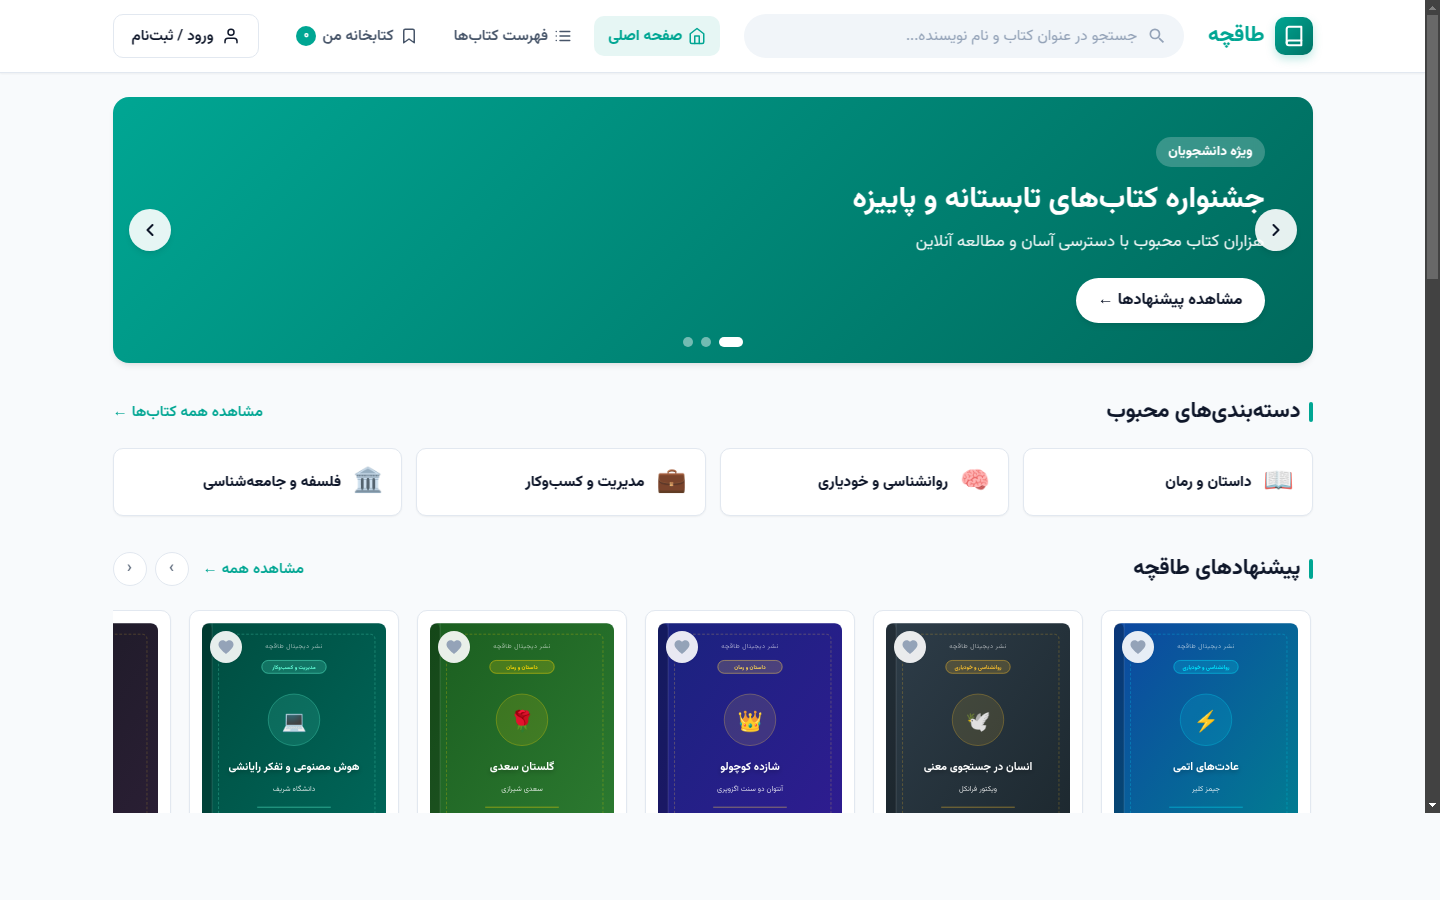
\includegraphics[width=0.48\textwidth]{assets/screenshots/screenshot-desktop-home.png}}
\hfill
\subfigure[نمای فهرست و فیلترهای کتاب‌ها]{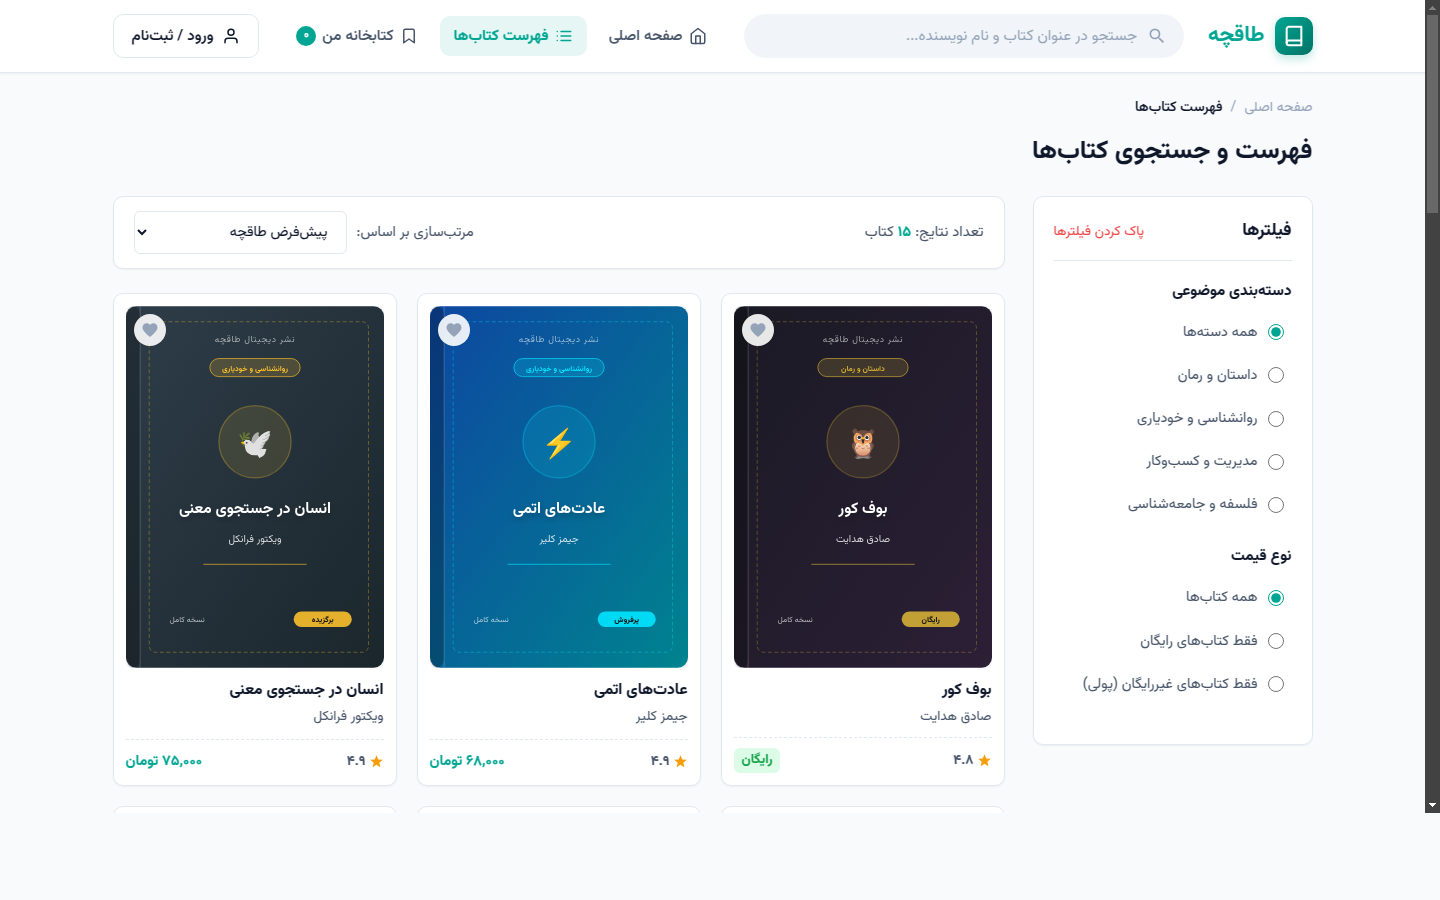
\includegraphics[width=0.48\textwidth]{assets/screenshots/screenshot-desktop-catalog.png}}
\\
\subfigure[نمای کتابخوان اختصاصی و تنظیمات متن]{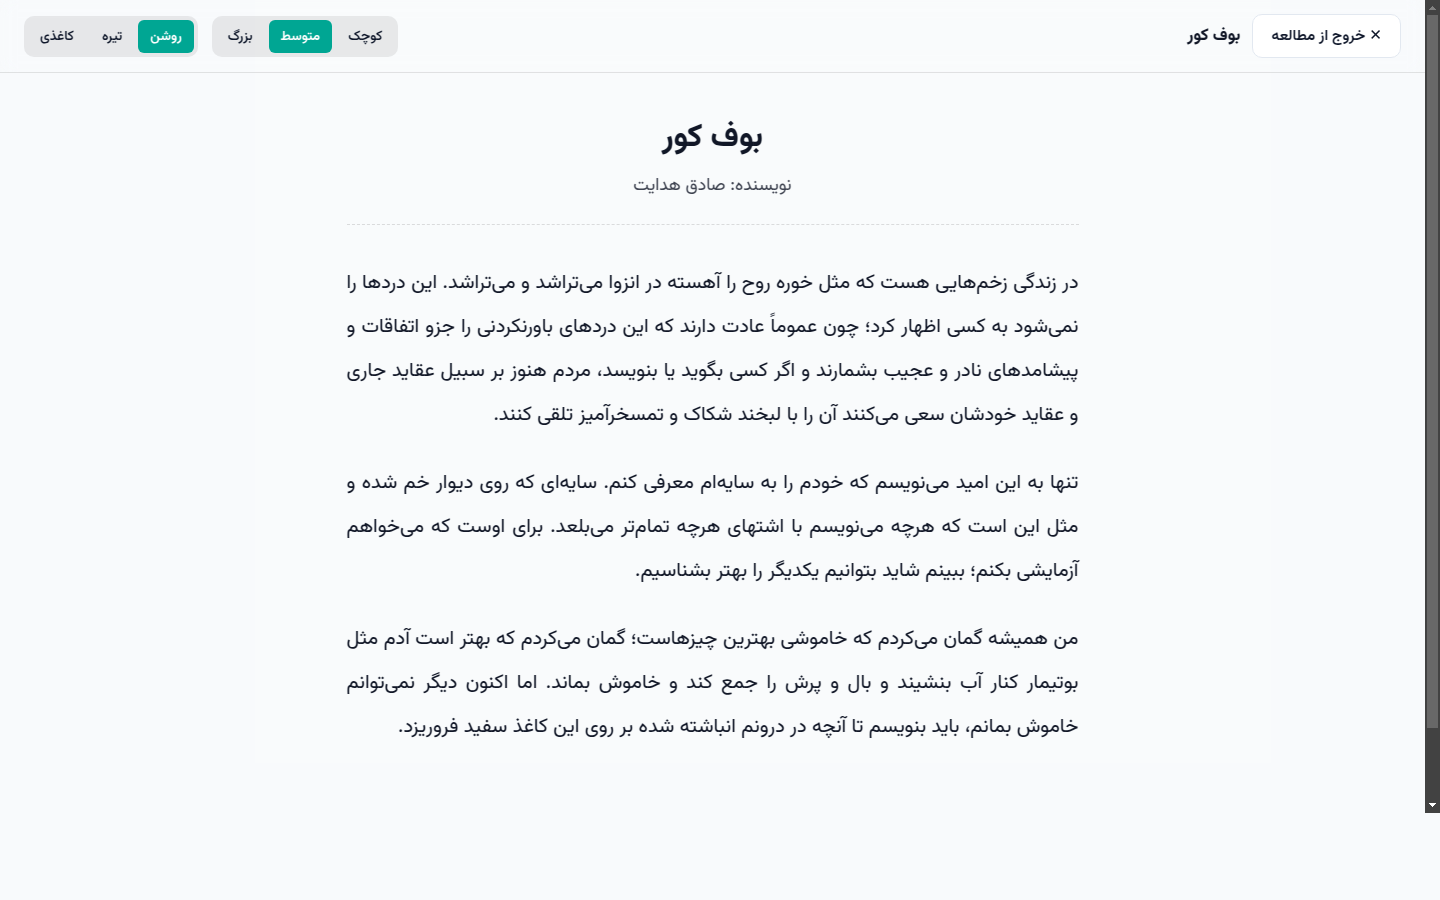
\includegraphics[width=0.48\textwidth]{assets/screenshots/screenshot-desktop-reader.png}}
\hfill
\subfigure[نمای واکنش‌گرا در موبایل (۳۶۰ پیکسل)]{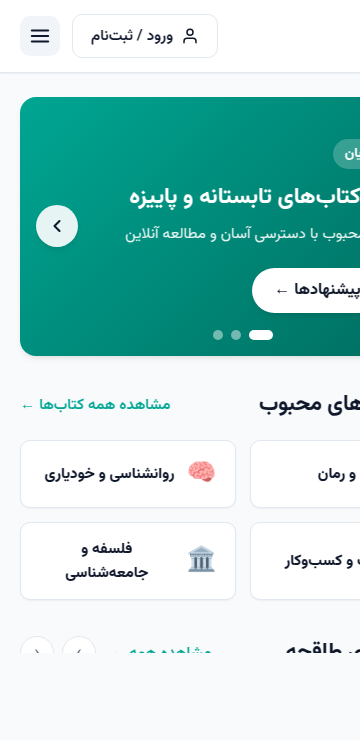
\includegraphics[width=0.48\textwidth]{assets/screenshots/screenshot-mobile.png}}
\caption{تصاویر خروجی وب‌اپلیکیشن پیاده‌سازی‌شده طاقچه در بخش‌های مختلف}
\end{figure}

\begin{itemize}
    \item \textbf{مراجع و ابزارها:} استانداردهای رسمی \lr{W3C} برای \lr{HTML5} و \lr{CSS3}، مستندات شبکه توسعه‌دهندگان موزیلا (\lr{MDN Web Docs})، تایپوگرافی متن‌باز \lr{Vazirmatn}، و چارچوب طراحی وب‌سایت اصلی طاقچه.
\end{itemize}

\end{questions}

\end{document}
